\section{Methoden}

Zu Lösung der Aufgabenstellung wird die sogenannte YOLO (\textit{You Only Look Once}) Netzstruktur in Python unter Nutzung der Keras API implementiert. YOLO Netze zeichnen sich durch gute Detektionsergebnisse bei einer sehr hohen Trainings- und Klassifikationsperfomanz aus. So ist mithilfe des YOLO-Modells sogar auf vergleichsweise kostengünstiger Hardware eine Echtzeitschätzung der Bounding-Boxen von Objekten möglich \cite{Redmon2016}. 

\subsection{Lossberechnung und Intersection over Union}
\label{Loss_ber}
Rezatofighi1 beschreibt die \textit{Intersection over Union} (IOU) als eine performante und präzise Möglichkeit den Loss bei der Objekterkennung zu bestimmen (s. Kap 2.2). Dabei wird die IOU aus dem Quotienten der sich überlappenden Fläche \textit{(Intersection / Overlap)} und der gemeinsam gebildeten Fläche (\textit{Union}) zweier Regionen berechnet: 
\begin{equation}\label{iou}
	IOU(y_{target},y_{pred})=\frac{y_{target} \cap y_{pred}}{y_{target} \cup y_{pred}}
\end{equation}
$y_{pred}$ steht hierbei für die geschätzte und $y_{target}$ für die reale Bounding-Box der Objekte. Die graphische Interpretation der Berechnung wird in Abbildung \ref{ioubild} deutlich. Zur Berechnung der jeweiligen Flächen wird der von Rezatofighil in \cite{Rezatofighi1902} beschriebene Algorithmus implementiert. Dort ist zusätzlich eine hier nicht genutzte Erweiterung zur \textit{Generalized-IOU} beschrieben.
\begin{figure}[!h]
  \centering
  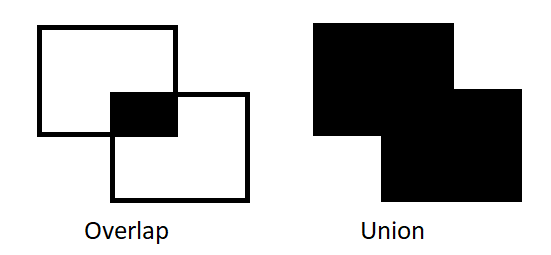
\includegraphics[width=8cm]{iou.png}
  \caption{Intersection over Union}
  \label{ioubild}
\end{figure} 
\FloatBarrier
Somit ergibt sich für den 2D-Fall als resultierende Loss-Funktion:
\begin{equation}\label{iouloss}
	L_{2D}= 1-IOU(y_{target},y_{pred})
\end{equation} 
Es ist darauf hinzuweisen, dass aufgrund der hohen Komplexität auf die Erweiterung der IOU Berechung für den 3D-Fall im Rahmen dieser Arbeit verzichtet wird. Möglich Ansätze für 3D-IOU Berechungen finden sich jedoch in \cite{Xu2019} und \cite{Mousavian1612}. Im 3D-Fall wird der Loss lediglich über den in Kapitel 2.2. beschriebenen L2-Ansatz bestimmt. In Abbildung \ref{L2_loss_graphik} ist schematisch dargestellt wie der L2 Loss berechnet wird. Hierfür wird lediglich der Abstand zwischen einem, vom Netz prädizierten Punkt und einem Zielpunkt berechnet. Dieser Abstand etspricht dem Ausdruck $y_{target}-y_{pred}$ aus Formel \ref{mse}. 
\begin{figure}[!htb]
  \centering
  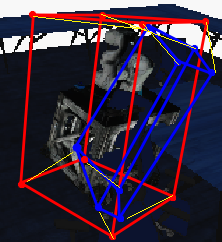
\includegraphics[width=6.2cm]{Abb/l2_loss_bei3d_bb.png}
  \caption{Prädizierte und gelabelte Punkte der Bounding-Box. Die gelben Linien stellen den Prädiktonsfehler dar}
  \label{L2_loss_graphik}
\end{figure} 
\newpage
\subsection{Netzstruktur}

\begin{figure}[!htb]
  \centering
  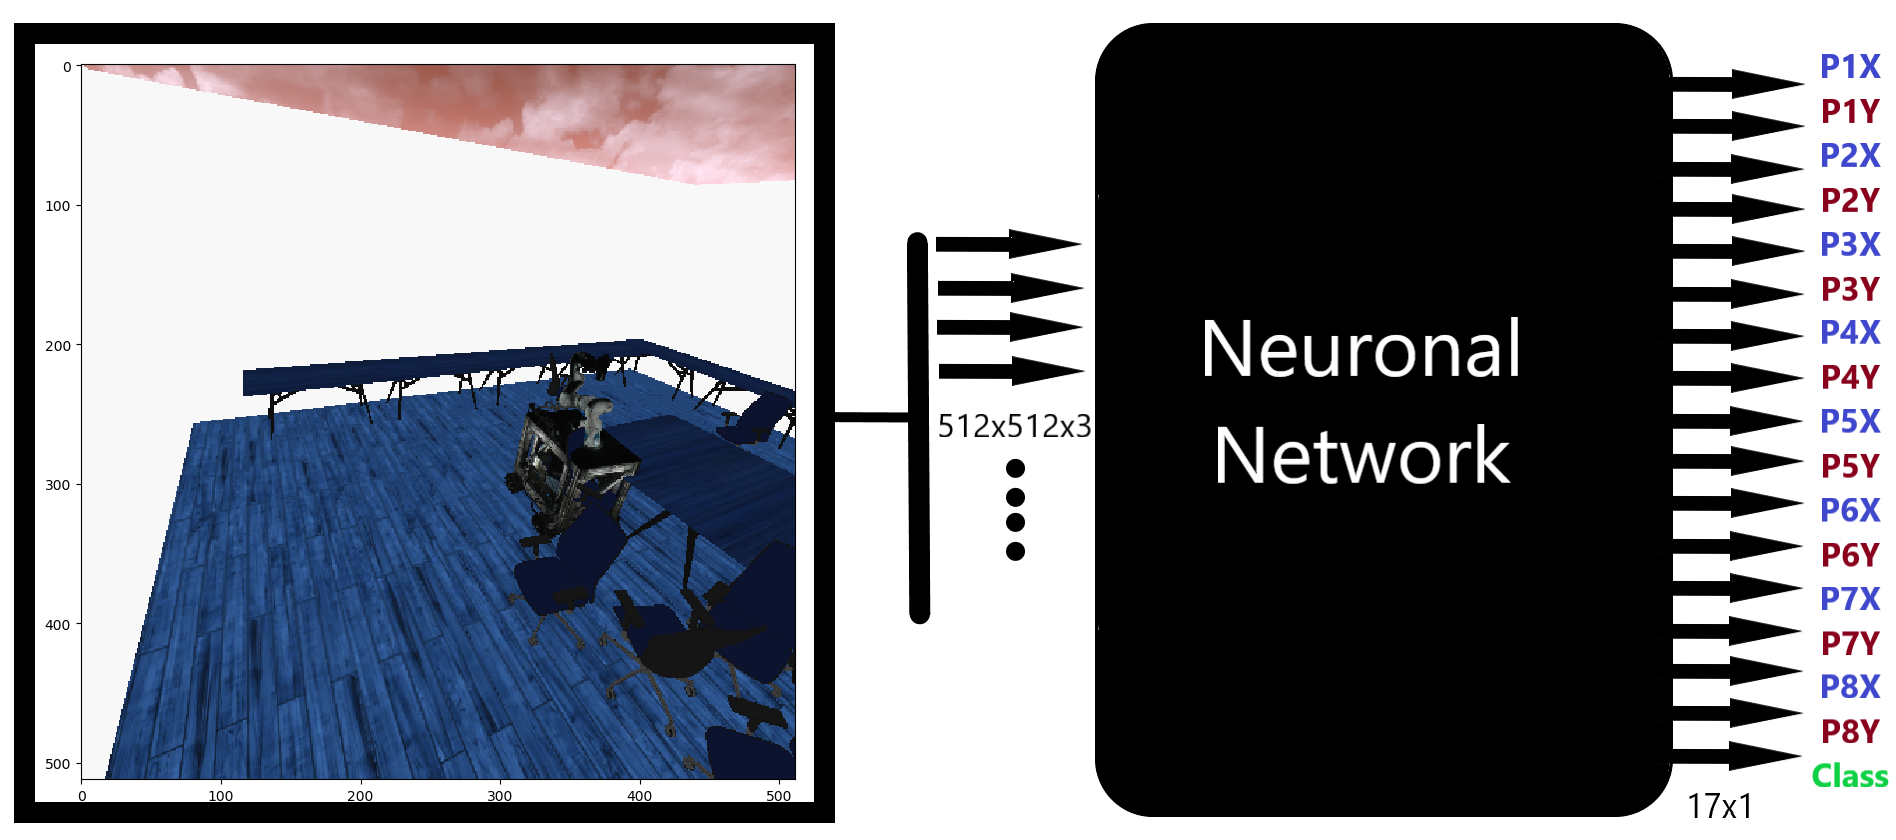
\includegraphics[width=13.8cm]{Abb/Modell_struktur.png}
  \caption{Grobe Darstellung der Netzstruktur zur prädiktion einer 3D Bounding-Box}
  \label{grobe_netz_struktur}
\end{figure} 

Die Netzstruktur, welche für die prädiktion einer 3D Bounding-Box verwendet wird orientiert sich sehr stark an dem sogenannten YOLO Netz. Die ersten Schichten des Netzes bestehen aus \textit{convolutional layern}, welche die Aufgabe haben Features aus dem Bild zu extrahieren. Die hintere Schicht des Netzes besteht aus  \textit{fully connected layern}, welche die Koordinaten der Bounding-Box Punkte sowie die Klassenzugehörigkeit  ausgeben \cite{Redmon2016}. \\Die Netzarchitektur muss jedoch für die Prädiktion einer projizierten 3D Bounding-Box angepasst werden. Diese besitzt im gegensatz zu einer 2D Bounding-Box 8 anstatt 2 erforderlichen Bildpunkten. Eine Vergleich einer 2D und einer 3D Bounding-Box ist in Abbildung \ref{3D_Bounding_roboter} aufgezeigt. Aus den 8 Punkten ergeben sich 16 Koordinaten. Zu den 16 Koordinaten kommt eine weitere Angabe über die Klasse des Objekts. Diese Angabe wird nur deshalb implementiert, um das Netz modularer und skalierbarer zu  machen. In dem hier behandelten Fall gibt es allerdings nur die eine Klasse namens \textit{Roboter}. in Abbildung \ref{grobe_netz_struktur} ist eine grobe Darstellung des implementierten Netzes als Blackbox dargestellt. Zu sehen sind die 17 Ausgänge, welche aus 16 Koordinaten für die Punkte der 3D Bounding-Box, sowie der Klassenzugehörigkeit bestehen. Im Anhang in Abbildung ... ist das Verwendete Netz detailliert dargestellt.

\begin{figure}[!htb]
  \centering
  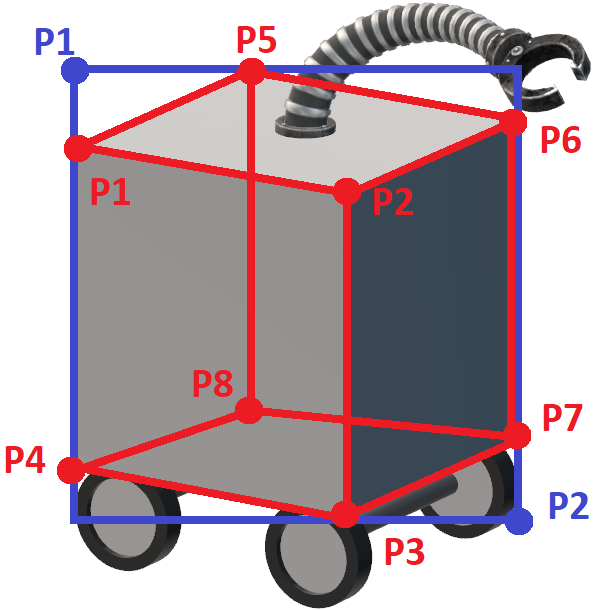
\includegraphics[width=6.8cm]{Abb/3d_robotter_mit_boundig_box_2d_vs_3d.PNG}
  \caption{3D Bounding-Box mit 8 Punkten \textcolor{red}{(rot)} und im Vergleich dazu eine 2D Bounding-Box mit 2 Punkten \textcolor{blue}{(blau)} }
  \label{3D_Bounding_roboter}
\end{figure} 

\newpage
\subsection{Training}
Für das Training wird ein gelabelter Datensatz verwendet, welcher vom Institut für eingebettete Systeme und Medizintechnik der Hochschule Mannheim bereitgestellt wird. Es liegen insgesamt 1000 gelabelte Samples vor, von denen 90\% für das Training und 10\% für die Validierung verwendet werden. Alle weiteren Trainingsparameter sind Tabelle \ref{trainings_param} zu entnehmen.\\

\begin{table}[!htb]

\centering
\caption{Trainingsparameter}
\begin{tabular}{ll}
\label{trainings_param}
\textbf{Parameters}                  & \textbf{Values} \\ \hline
\\Convolutional Layer        & 9      \\
Fully connected Layer       & 2      \\
Anzahl der Trainingssamples & 900    \\
Epochen                  & 15     \\
Batch Size                  & 1     \\
Optimizer                   & Adam   \\
Learning Rate               & 0,0001 \\
Loss Function               & MSE (siehe \ref{Loss_ber})   
\end{tabular}
\end{table}
Auf einer NVIDIA GTX9600M Grafikkarte mit mit einer \textit{NVIDIA Compute Capability} von 5, benötigt das Training des Netzwerks zur Detektion einer 3D Bouding box lediglich 12 Minuten.
  
\subsection{Softwaremodul Beschreibung}
Für die Realisierung eines Netzwerkes zu Bestimmung einer 3D Bounding-Box werden einige Softwaremodule implementiert. Im folgenden werden diese Module beschrieben. 
\subsubsection{Laden der Daten}
Das laden der Trainingsdaten wird durch eine eigens dafür entwickelte klasse Implementiert. Die Bilder liegen im .png Format und die Labls im .json Format vor. Die Klasse lädt diese Daten, teilt diese in Trainings- und Testdaten auf und gibt die Daten als \textit{numpy arrays} zurück, sodass diese direkt für das Training verwendet werden können. In Abbildung \ref{UML_load} ist das zu der Klasse gehörige UML Diagramm mit allen Methoden aufgezeigt.
\begin{figure}[!htb]
  \centering
  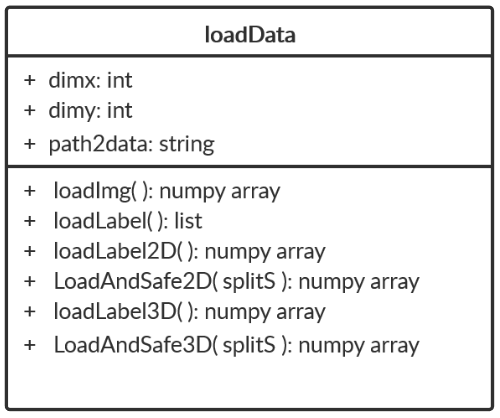
\includegraphics[width=6.8cm]{Abb/ULM_class_loadData.PNG}
  \caption{UML Diagramm loadData}
  \label{UML_load}
\end{figure} 
\subsubsection{Objekt Lokalisierung}
in der Klasse \textit{ObjectLocalizer3D} befindet sich der für das Neuronale Netz relevante Programmcode. Hier wird unter anderem das Netz erzeugt, die Loss Funktion definiert, sowie eine Metrik geschrieben. Die Klasse ist abgeleitet von der \textit{Keras functional API}. Die Klasse besitzt auch Methoden, wie fit, welche direkt auf die zu der \textit{Keras functional API} zugehörige fit Methode zugreift. Ebenfalls ist es möglich die Trainierten Modelle zu speichern oder diese zu Laden. In Abbildung \ref{UML_localizer} ist ein UML Diagramm der Klasse dargestellt.  
\begin{figure}[!htb]
  \centering
  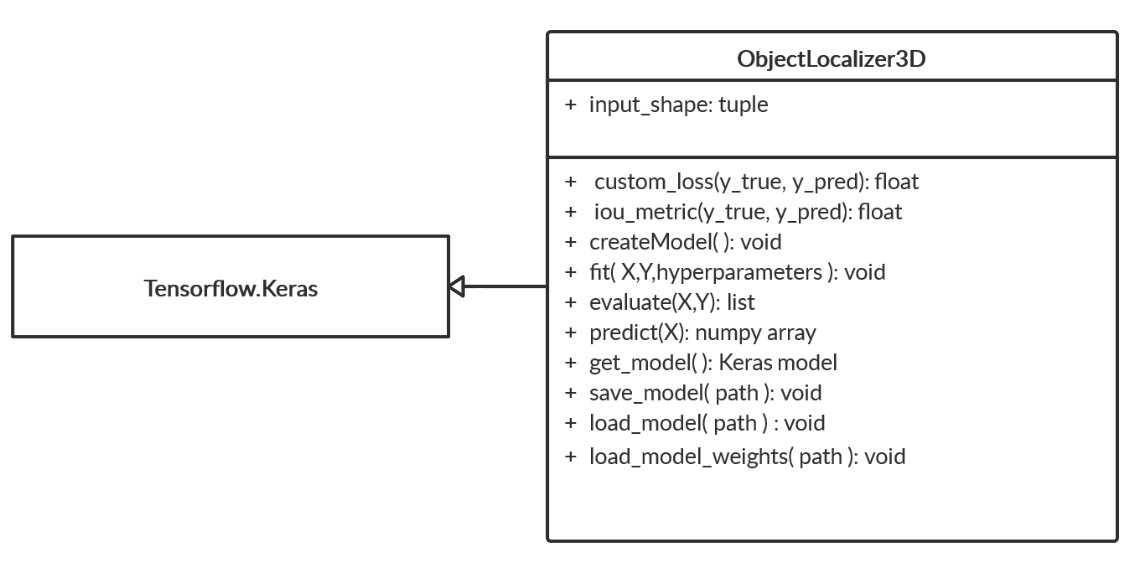
\includegraphics[width=13.8cm]{Abb/ULM_class_objectLocalizer.PNG}
  \caption{UML Diagramm der Klasse ObjectLocalizer3D, welche von der \textit{Keras functional API} abgeleitet ist}
  \label{UML_localizer}
\end{figure} 
\newpage

  